\documentclass[%
reprint,
superscriptaddress,
%groupedaddress,
%unsortedaddress,
%runinaddress,
%frontmatterverbose,
%preprint,
showpacs,preprintnumbers,
%nofootinbib,
%nobibnotes,
%bibnotes,
 amsmath,amssymb,
 aps,
%pra,
%prb,
prd,
%prl,
%rmp,
%prstab,
%prstper,
%floatfix,
]{revtex4-1}

\usepackage{float}
\usepackage{graphicx}% Include figure files
\usepackage{dcolumn}% Align table columns on decimal point
\usepackage{bm}% bold math
\usepackage{bbold}
\usepackage{amssymb,amsmath}
\usepackage{hyperref}% add hypertext capabilities
%\usepackage[mathlines]{lineno}% Enable numbering of text and display math
%\linenumbers\relax % Commence numbering lines

%\usepackage[showframe,%Uncomment any one of the following lines to test
%%scale=0.7, marginratio={1:1, 2:3}, ignoreall,% default settings
%%text={7in,10in},centering,
%%margin=1.5in,
%%total={6.5in,8.75in}, top=1.2in, left=0.9in, includefoot,
%%height=10in,a5paper,hmargin={3cm,0.8in},
%]{geometry}



\usepackage{color}
\usepackage{amsfonts}
\usepackage{subfigure}
\usepackage{array}


\newcommand{\Tr}{\ensuremath{\operatorname{Tr}}}
\newcommand{\tr}{\ensuremath{\operatorname{tr}}}
\newcommand{\Omegaqq}{\ensuremath{\Omega_{\bar{q}q}}}
\newcommand{\vev}[1]{\ensuremath{\left\langle #1 \right\rangle}}
\newcommand{\einh}[1]{\ensuremath{\,\text{#1}}}
\newcolumntype{L}{>{\centering\arraybackslash}m{3cm}}



\newcommand{\overbar}[1]{\mkern 1.5mu\overline{\mkern-1.5mu#1\mkern-1.5mu}\mkern 1.5mu}

\definecolor{bjcol}{rgb}{1,.44,0.13}

% color def's

\definecolor{blue}{rgb}{0,0,1}
\newcommand{\colb}[1]{{\color{blue} #1}}
\definecolor{green}{rgb}{0,1,0}
\newcommand{\colg}[1]{{\color{green} #1}}
\definecolor{red}{rgb}{1,0,0}
\newcommand{\colr}[1]{{\color{red} #1}}
\newcommand{\colJ}[1]{{\color{cyan} #1}}
\definecolor{gray}{rgb}{.5,.5,.5}
\newcommand{\drop}[1]{{\sout{ {\color{gray} #1}}}}
\definecolor{darkgreen}{rgb}{.0,.5,.0}
\newcommand{\colL}[1]{{\color{darkgreen} #1}}


\def\Fig#1{Fig.~\ref{#1}} \def\Tab#1{Tab.~\ref{#1}}
\def\Figs#1{Figs.~\ref{#1}} \def\Tab#1{Tab.~\ref{#1}}
\def\Eqs#1{Eqs.~(\ref{#1})}
\def\Eq#1{Eq.~(\ref{#1})}
\def\eq#1{(\ref{#1})}
\def\eqref#1{(\ref{#1})}
\def\fig#1{Fig.~\ref{#1}}
\def\tab#1{Tab.~\ref{#1}}
\def\eqs#1{(\ref{#1})}
\def\Eqs#1{(\ref{#1})}
\def\sec#1{Sec.~\ref{#1}}
\def\app#1{Appendix~\ref{#1}}
\newcommand{\Phibar}{\ensuremath{\bar{\Phi}}}
\newcommand{\LPQM}{\ensuremath{\mathcal{L}_{\textrm{PQM}}}\xspace}

\def\dbar{{\mathchar'26\mkern-12mu d}}
\def\lA0{{\langle A_0 \rangle}}
\def\bA0{{\bar{A}_0}}
\def\lLA{{\langle L[A_0] \rangle}}
\def\lL{{\langle L \rangle}}
\def\lLc{{\langle L^\dagger \rangle}}
\def\lLAc{{\langle L^\dagger[A_0] \rangle}}


\def\dr{{D\!\llap{/}}\,}
\def\Dr{{D\!\llap{/}}\,}
\def\ipv{\vec{p}\llap{/}}
\def\pslash{p\llap{/}}

\def\0#1#2{\frac{#1}{#2}}

\newcommand{\bsig}{\ensuremath{\bar{\sigma}}}
\newcommand{\lsm}{L\ensuremath{\sigma}M\xspace}
\newcommand{\pT}{\ensuremath{T_0}}
\newcommand{\Tl}{\ensuremath{T_\chi}}
\newcommand{\Ts}{\ensuremath{T_\chi^s}}
\newcommand{\Tchi}{\ensuremath{T_\chi}}
\newcommand{\Td}{\ensuremath{T_d}}
\newcommand{\Tc}{\ensuremath{T_c}}
\newcommand{\muc}{\ensuremath{\mu_c}}
\newcommand{\coloronl}{(color online)\xspace}

\newcommand{\mrm}[1]{\mathrm{#1}}
\def\qbar{\bar{q}}
\newcommand{\sx}{\sigma_{x}}
\newcommand{\sy}{\sigma_{y}}

%%%%%%%%%%%%%% for corrections %%%%%%%%%%%
\newcommand{\colsy}[1]{\textcolor{blue}{#1}}
\newcommand{\colrw}[1]{\textcolor{cyan}{#1}}
\newcommand{\colwjf}[1]{\textcolor{red}{#1}}

%
%%%%%%%%%%%%%%%%%%%%%%%%%%%%%%%%%%%%%%%%%%%%%%%%%%%%%%%%%%%%%%%%%%%%%%%%%%%%%

\graphicspath{{./figures/}{./}}

\begin{document}

\preprint{}

\title{Mesonic dynamics and QCD phase transition
}

\author{Shi Yin}
\affiliation{School of Physics, Dalian University of Technology, Dalian, 116024,
  P.R. China}

\author{Rui Wen}
\affiliation{School of Physics, Dalian University of Technology, Dalian, 116024,
  P.R. China}

\author{Wei-jie Fu}
\email{wjfu@dlut.edu.cn}
\affiliation{School of Physics, Dalian University of Technology, Dalian, 116024,
  P.R. China}

%\date{\today}% It is always \today, today,
             %  but any date may be explicitly specified

\begin{abstract}
We study the finite temperature and density two flavor quark-meson model under the functional renormalisation group. The effect of broken $O(4)-$ symmetry of the wave function  renormalisation and expansion point of effective potential on the thermodynamic quantities and baryon number fluctuation are investigate. At the same time, the field dependent Yukawa coupling is also considered. We give results of the pion mass, the quark mass, the trace anomaly, the baryon number fluctuation and the freeze-out curve.
\end{abstract}

%\pacs{Valid PACS appear here}% PACS, the Physics and Astronomy
%\pacs{11.30.Rd, %Chiral symmetries
%         11.10.Wx, %Finite-temperature field theory
%        05.10.Cc, %Renormalization group methods
%         12.38.Mh  %Quark-gluon plasma
%     }                             % Classification Scheme.
%\keywords{Suggested keywords}%Use showkeys class option if keyword
                              %display desired
\maketitle

%\tableofcontents

%%%%%%%%%%%%%%%%%%%%%%%%%%%%%%%%%%%%%%%%%%%%%%%%%%%%%%%%%%%
%%%%%%%%%%%%%%%%%%%%%%%%%%%%%%%%%%%%%%%%%%%%%%%%%%%%%%%%%%%

\section{Introduction}
\label{sec:int}


The QCD phase structure and the search of the critical end point (CEP) are the most popular research direction in both experimental and theoretical field. The phase transition between the quark gluon plasma (QGP) and hadron is the main research objects. The research of the QGP-hadron phase transition can help us to help us better understand the nature of elementary particles. The experiment to looking for the QGP is being made at the Large Hadron Collider (LHC) and the Relativistic Heavy-Ion Collider (RHIC).

In terms of theoretical research, there many different methods to investigate the QCD phase structure. The most widely studied method is the lattice QCD. A lot of properties of the QCD matter have been discussed under the lattice simulations. Although the lattice theory has the sign problem at high baryon chemical potential, it still gave us plenty of great outcomes. In order to avoid the problem that occurs in lattice calculation, the study of the continuous non-perturbative field theory is in progress at the same time. For example, the Dyson-Schwinger equation. And the Functional Renormalization Group (FRG) is the other good functional approach of the continuous theory. In these ways we can study the behavior of the strong interaction matter under the finite temperature and density better.

This work is done with the low energy effective model under the FRG approach. 
%%%%%%%%%%%%%%%%%%%%%%%%%%%%%%%%%%%%



The low-energy effective models, e.g. the quark-meson (QM) model \cite{Schaefer:2004en}, Nambu--Jona-Lasinio (NJL) model, and their Polyakov-loop improved variants: PQM and PNJL, are suitable to be employed to study the QCD phase transitions. They have been investigated quite a lot in literatures, see, e.g., \cite{} for more details. In this work, we adopt the scale-dependent effective action for the two-flavor PQM model, as follows 
\begin{align}
\Gamma_k=&\int_x \bigg\{Z_{q,k}\bar{q} \Big [\gamma_\mu \partial_\mu -\gamma_0(\hat\mu+igA_0) \Big ]q \nonumber\\[2ex]
&+\frac{1}{2}\Big [Z_{\phi,k}^{\parallel}(\partial_0 \phi)^2+Z_{\phi,k}^{\perp}(\partial_i \phi)^2 \Big]\nonumber\\[2ex]
&+h_k(\rho)\bar{q}\big(T^0\sigma+i\gamma_5\vec{T}\cdot \vec{\pi}\big)q+V_k(\rho)-c\sigma \bigg\}\,,\label{eq:action}
\end{align}
with $\mu=(0, 1, ..., 3)$ and $i=(1, 2, 3)$. In \Eq{eq:action} we have used notation $\int_{x}=\int_0^{1/T}d x_0 \int d^3 x$, where the imaginary time formalism for the field theory at finite temperature is used, and the temporal length reads $\beta=1/T$. Apparently, when the temperature is nonzero, the $O(4)$-symmetry in the Euclidean space is broken into that of $\mathbb{Z}_2\otimes O(3)$, which leads to the split of the magnetic and electric components of correlations functions. They correspond to the components transversal and longitudinal to the heat bath, respectively. In this work, we take this split into account in the two-point correlation function for the mesons, as shown in the second line on the r.h.s. of \Eq{eq:action}, where $Z_{\phi,k}^{\parallel}$ and $Z_{\phi,k}^{\perp}$ indicate the longitudinal and transversal wave function renormalizations for the temporal and spacial components, respectively. 

The reason why we concentrate on the split of the wave function renormalization especially for the mesons is due to the facts as follows. Firstly, in comparison to the quark wave function renormalization $Z_{q,k}$ and the scale dependent Yukawa coupling $h_k$ in \Eq{eq:action}, it is found that the meson wave function renormalization $Z_{\phi,k}$ plays the most significant role beyond the local potential approximation (LPA) \cite{Pawlowski:2014zaa,Fu:2015naa}. In the LPA, the propagators are classical, i.e., $Z_{q,k}=Z_{\phi,k}=1$ and the Yukawa coupling $h$ is a constant and independent of the scale $k$. Secondly, In Ref. \cite{Helmboldt:2014iya} calculations based on the full momentum-dependent two-point correlation functions of mesons are compared with those from LPA and LPA$'$, and here in LPA$'$ a momentum-independent $Z_{\phi,k}$ is included, and it is found that there is a good agreement between the full momentum calculation and the LPA$'$, while not LPA, which indicates that the dispersion relation for the meson, resulting from a scale dependent $Z_{\phi,k}$, have already captured most momentum dependence of the two-point correlation function. 

Considering the importance of the wave function renormalization for the mesons and the success of LPA$'$, in this work we would like to investigate the effects of the splitting of $Z_{\phi,k}$ in the LPA$'$ as shown in \Eq{eq:action}, which is a natural choice at finite temperature as discussed above. Furthermore, we will also study the interplay between the splitting of $Z_{\phi,k}$ and other truncation approaches, e.g., the field dependent Yukawa coupling $h_k(\rho)$ which encodes higher order quark-meson scattering processes \cite{Pawlowski:2014zaa}, fixed point expansion for the effective potential $V_k(\rho)$ in \Eq{eq:action} versus the physical point expansion, etc. Their influences on the QCD phase transition and observables, e.g. fluctuations of the baryon number, will be investigated in detail.


%%%%%%%%%%%%%%%%%%%%%%%%%%%%%%%%%%%%%%%%%%%%%%%%%%%%%%%%%%%%%
%%%%%%%%%%%%%%%%%%%%%%%%%%%%%%%%%%%%%%%%%%%%%%%%%%%%%%%%%%%%%

\section{Functional renormalization group and flow equations}
\label{sec:FRG}

To proceed, we describe other notations in the effective action in \Eq{eq:action}. $\phi=\left(\sigma,\vec{\pi}\right)$ is a meson field with four components. The effective potential $V_k(\rho)$ with $\rho=\phi^2/2$ is $O(4)$ invariant and the c-term $c\sigma$ breaks the chiral symmetry explicitly. The mesons interact with quarks through the scalar and pseudo-scalar channels with a mesonic field dependent Yukawa coupling $h_k(\rho)$, and $T^0$ and $T^i$ are the generators in the flavor space with the convention as follows: $\Tr(T^{i}T^{j})=\frac{1}{2}\delta^{ij}$ and $T^{0}=\frac{1}{\sqrt{2N_{f}}}\mathbb{1}_{N_{f}\times N_{f}}$ with $N_{f}=2$. Besides the wave function renormalization for the meson, we also introduce one for the quark, i.e., $Z_{q,k}$. Since it plays a minor role in the chiral dynamics in comparison to $Z_{\phi,k}$, the splitting of $Z_{q,k}$ into the transversal and longitudinal components are neglected for simplicity in calculations. Finally, $\hat\mu=\mathrm{diag}(\mu_u,\mu_d)$ in the first line on the r.h.s. of \Eq{eq:action} denotes the matrix of the quark chemical potential, and $\mu=\mu_u=\mu_d$ is assumed in the following unless stating specifically. $A_0$ is the temporal gluon background field, through which the Polyakov dynamics is taken into account.

The renormalization group (RG) scale $k$ in \Eq{eq:action} is an infrared cutoff, below which quantum fluctuations are suppressed in the effective action. The evolution of the effective action with $k$ is described by the Wetterich equation \cite{Wetterich:1992yh}, which reads 
\begin{align}
  \partial_t\Gamma_k[\Phi]&=\frac{1}{2}\mathrm{Tr}\big(G_{\phi\phi,k}\partial_t R^{\phi}_{k}\big)-\mathrm{Tr}\big(G_{q\bar{q},k}\partial_t R^{q}_{k}\big)\,, \label{eq:WetterichEqPQM}
\end{align}
with the RG time $t=\ln (k/\Lambda)$ and the initial ultraviolet (UV) cutoff $\Lambda$, where $R^{\phi}_{k}$ and $R^{q}_{k}$ are the regulators for the meson and quark fields, respectively, and they are given in Eqs.~(\ref{eq:Rphi}) and ~(\ref{eq:Rq}). The scale dependent meson and quark propagators are given by
\begin{align}
  G_{\phi\phi/q\bar{q}}[\Phi]=\left( \frac{1}{\frac{\delta^2\Gamma_k[\Phi]}{\delta\Phi^2}+R^{\Phi}_{k}} \right)_{\phi\phi/q\bar{q}}\,, \label{eq:props}
\end{align}
with $\Phi=(q,\bar q,\phi)$ denoting all species of fields.

Inserting the effective action in \Eq{eq:action} into the flow equation \eq{eq:WetterichEqPQM}, one arrives at the flow equation for the effective potential, which reads
\begin{align}
  \partial_t V_k(\rho)=&\frac{k^4}{4\pi^2} \bigg [\big(N^2_f-1\big) l^{(B,4)}_{0}(\bar{m}^{2}_{\pi,k},\eta^{\perp}_{\phi,k},z_\phi;T)\nonumber\\[2ex]
&+l^{(B,4)}_{0}(\bar{m}^{2}_{\sigma,k},\eta^{\perp}_{\phi,k},z_\phi;T)\nonumber\\[2ex]
&-4N_c N_f l^{(F,4)}_{0}(\bar{m}^{2}_{q,k},\eta_{q,k};T,\mu)\bigg]\,, \label{eq:flowV}
\end{align}
with the RG invariant dimensionless meson and quark masses as follows
\begin{align}
  \bar{m}^{2}_{\pi,k}&=\frac{V'_k(\rho)}{k^2Z^{\perp}_{\phi,k}}\,, \qquad \bar{m}^{2}_{\sigma,k}=\frac{V'_k(\rho)+2\rho V''_k(\rho)}{k^2 Z^{\perp}_{\phi,k}}\,,\\[2ex]
  \bar{m}^{2}_{q,k}&=\frac{h^{2}_{k}\rho}{2k^2Z^{2}_{q,k}}\,.
\end{align}
The threshold functions $l^{(B)}_{0}$ and $l^{(F)}_{0}$ are presented in Eqs. (\ref{eq:l0B}) and (\ref{eq:l0F}), and the anomalous dimensions for the mesons and quark are defined as
\begin{align}
  \eta_{\phi,k}^{\perp}&=-\frac{\partial_t Z_{\phi,k}^{\perp}}{Z_{\phi,k}^{\perp}}\,,\quad \eta_{\phi,k}^{\parallel}=-\frac{\partial_t Z_{\phi,k}^{\parallel}}{Z_{\phi,k}^{\parallel}}\,,\quad \eta_{q,k}=-\frac{\partial_t Z_{q,k}}{Z_{q,k}}\,. \label{}
\end{align}
Note that $z_\phi \equiv Z_{\phi,k}^{\parallel}/Z_{\phi,k}^{\perp}$ enters into the flow of $V_k(\rho)$ through the mesonic fluctuations as shown in \Eq{eq:flowV}. 

The transversal anomalous dimension for the  $\pi$-meson is obtained by employing the projection as follows
\begin{align}
  \eta_{\phi,k}^{\perp}&=-\frac{1}{3Z_{\phi,k}^{\perp}}\delta_{ij}\frac{\partial}{\partial (|\bm{p}|^2)}\frac{\delta^2 \partial_t \Gamma_k}{\delta \pi_i(-p) \delta \pi_j(p)}\Bigg|_{\substack{p_0=0\\ \bm{p}=0}}\,,\label{eq:etaphiperp}
\end{align}
and the longitudinal one reads
\begin{align}
  \eta_{\phi,k}^{\parallel}&=-\frac{1}{3Z_{\phi,k}^{\parallel}}\delta_{ij}\frac{\partial}{\partial (p_0^2)}\frac{\delta^2 \partial_t \Gamma_k}{\delta \pi_i(-p) \delta \pi_j(p)}\Bigg|_{\substack{p_0=0\\ \bm{p}=0}}\,.\label{eq:etaphipara}
\end{align}
Their explicit expressions are given in Eqs. (\ref{eq:etaphiperp2}) and (\ref{eq:etaphipara2}), respectively. The difference of the anomalous dimension between the $\pi$ and $\sigma$ mesons is neglected here. Note that even they are different, choosing the $\pi$-meson anomalous dimension for $\eta_\phi$, as done in this work, could minimize the errors of calculation, at least when the baryon chemical potential is not very high, since the mass of the pion is less than that of $\sigma$-meson, because of its nature of Goldstone particle, and the number of the degree of freedom for the pion is also larger. But we should mention that, in the region of the high baryon chemical potential in the phase diagram, especially near the CEP, the $\sigma$-mode is the most relevant collective mode and the mass of the $\sigma$-meson is vanishing, it is necessary to distinguish the anomalous dimensions of $\pi$ and $\sigma$, which will be investigated in the future.

The anomalous dimension for the quark is obtained by projecting the inverse quark propagator onto the vector channel, as follows
\begin{align}
  \eta_{q}&(p_0,\bm{p})=\frac{1}{4 Z_{q,k}(p_0,\bm{p})}\nonumber \\[2ex]
          &\times\mathrm{Re}\left[\frac{\partial}{\partial (|\bm{p}|^2)}\mathrm{tr}
            \left(i \bm{\gamma}\cdot\bm{p}\left(-\frac{\delta^2}{\delta\bar{q}(p)
            \delta q(p)}\partial_t \Gamma_k\right)\right)\right]\Bigg|_{\substack{p_{0,ex}\\ \bm{p}=0}}\,.   \label{eq:etapsi}
\end{align}
where the spacial component of the external momentum is chosen to be vanishing, as same as the mesonic anomalous dimensions in Eqs. (\ref{eq:etaphiperp}) and (\ref{eq:etaphipara}). Note that because of the fermionic property of the quark, its lowest Matsubara frequency is nonvanishing, and we denote it here as $p_{0,ex}$, which is described in \app{app:anom}.  Projecting of the inverse quark propagator onto the scalar channel leads us to the flow of the Yukawa coupling \cite{Pawlowski:2014zaa}, which reads
\begin{align}
  \partial_t h_k(\rho)&=\frac{1}{2 \sigma}\mathrm{Re}\left[\mathrm{tr}\left(-\frac{\delta^2}{\delta\bar{q}(p)
            \delta q(p)}\partial_t \Gamma_k\right)\right]\Bigg|_{\substack{p_{0,ex}\\ \bm{p}=0}}\,.  \label{eq:dth}
\end{align}
The analytic expressions of \Eq{eq:etapsi} and \Eq{eq:dth} are given in \Eq{eq:etapsi2} and \Eq{eq:dth2}, respectively.


%%%%%%%%%%%%%%%%%%%%%%%%%%%%%%%%%%%%%%%%%%%%%%%%%%%%%%%%%%%%%
%%%%%%%%%%%%%%%%%%%%%%%%%%%%%%%%%%%%%%%%%%%%%%%%%%%%%%%%%%%%%

\section{Equation of state and baryon number fluctuations}
\label{sec:EoS}

In the PQM model (\ref{eq:action}) the thermodynamical potential density reads
\begin{align}
  \Omega[T,\mu]&=V_{k=0}(\rho)-c\sigma+V_{\text{\tiny{glue}}}(L, \bar L)\,,\label{eq:omega}
\end{align}
where all the fields are on their respective equations of motion. $L$ is the traced Polyakov loop and $\bar L$ is its complex conjugate. They are related to the temporal gluonic background field $A_0$ in \Eq{eq:action} through the equations as follows
\begin{align}
L(\bm x)=\frac{1}{N_c}\langle \Tr{\mathcal{P}(\bm x)} \rangle ,\qquad \bar{L} (\bm x)=\frac{1}{N_c}\langle \Tr{\mathcal{P}^{\dagger}(\bm x)} \rangle\,,\label{}
\end{align}
with the Polyakov loop $\mathcal{P}(\bm x)$ which reads
\begin{align}
\mathcal{P}(\bm x)=\mathcal{P}\exp\bigg( ig\int_{0}^{\beta}d\tau A_0(\bm x,\tau) \bigg)\,,\label{}
\end{align}
where the path-ordering operator $\mathcal{P}$ has been employed.

In this work we employ the polynomial parametrization of the glue potential \cite{Ratti:2005jh}, which reads 
\begin{align}
  \bar V_{\text{\tiny{glue}}}(L,\bar L)=& -\frac{b_2(T)}{2}L\bar{L}-\frac{b_3}{6}(L^3+\bar{L}^3)+\frac{b_4}{4}(L\bar{L})^2\,,\label{eq:Glueppoly}
\end{align}
with the dimensionless glue potential $\bar V_{\text{\tiny{glue}}}=V_{\text{\tiny{glue}}}/T^4$. The temperature dependence of the glue potential is encoded in the coefficient of the quadratic term in the Polyakov loop, to wit,
\begin{align}
  b_2(T)&=a_1+\frac{a_2}{1+t_r}+\frac{a_3}{(1+t_r)^2}+\frac{a_4}{(1+t_r)^3}\,,\label{eq:b2}
\end{align}
with the reduced temperature $t_r=(T-T_c)/T_c$. The parameters in the glue potential are determined by fitting the thermodynamics and the Polyakov loop dynamics in the Yang-Mills (YM) theory, which are $a_1=6.75$, $a_2=-1.95$, $a_3=2.625$, $a_4=-7.44$,  $b_3=0.75$, and $b_4=7.5$. It has been found that the unquenched effect on the glue potential in QCD is well captured from that in the YM theory \cite{Haas:2013qwp}, by employing the rescale for the reduced temperature as follows
\begin{align}
  (t_r)_{\text{\tiny{YM}}}&\rightarrow \alpha\,(t_r)_{\text{\tiny{glue}}}\,,\label{}
\end{align}
with
\begin{align}
  (t_r)_{\text{\tiny{glue}}}&=(T-T_c^\text{\tiny{glue}})/T_c^\text{\tiny{glue}}\,,\label{}
\end{align}
and $\alpha \simeq 0.57$. In this work we adopt $T_c^\text{\tiny{glue}}=208$ MeV for $N_f=2$ flavor QCD, which is obtained from the renormalization group analysis in QCD, see \cite{Schaefer:2007pw} for details.

The pressure and the energy density are given by
\begin{align}
  p&=-\Omega[T,\mu]\,,\\[2ex]
 \varepsilon&=-p+Ts +\sum_{i=u,d}\mu_i n_i\,,\label{}
\end{align}
with the entropy density and quark number density reading 
\begin{align}
  s&=\frac{\partial p}{\partial T}\qquad \text{and}\qquad n_i=\frac{\partial p}{\partial \mu_i}\,,\label{}
\end{align}
respectively. The interaction measure or the trace anomaly is given as follows
\begin{align}
  \Delta&=\varepsilon-3p\,.\label{}
\end{align}

In this work we will also investigate the fluctuations of the baryon and quark numbers, which are obtained through high-order derivatives of the pressure w.r.t. their respective chemical potentials. Taking the baryon number fluctuations for instance, the $n$-th order one reads
\begin{align}
   \chi_n^{B}&=\frac{\partial^n}{\partial (\mu_B/T)^n}\frac{p}{T^4}\,,\label{eq:suscept}
\end{align}
which is also called as the $n$-th order generalized susceptibility of the baryon number. $ \chi_n^{B}$'s in \Eq{eq:suscept} are related to the cumulants of the baryon number distributions, e.g.,
\begin{align}
  \chi_1^B&=\frac{1}{VT^3}\langle N_B \rangle\,,\\[2ex]
  \chi_2^B&=\frac{1}{VT^3}\langle(\delta N_B)^2\rangle\,,\\[2ex]
  \chi_3^B&=\frac{1}{VT^3}\langle(\delta N_B)^3\rangle\,,\\[2ex]
  \chi_4^B&=\frac{1}{VT^3}\Big(\langle(\delta N_B)^4\rangle-3\langle(\delta N_B)^2\rangle^2\Big)\,,
\end{align}
up to the fourth order. Here $\langle ...\rangle$ denotes the ensemble average and $\delta N_B=N_B-\langle N_B\rangle$. These generalized susceptibilities are related to the cumulants of the baryon number distribution in the experiments, such as the mean value $M=VT^3\chi_1^{B}$, the variance $\sigma^2=VT^3\chi_2^{B}$, the skewness $S=\chi_3^{B}/(\chi_2^{B}\sigma)$, and the kurtosis $\kappa=\chi_4^{B}/(\chi_2^{B}\sigma^2)$, etc.


%%%%%%%%%%%%%%%%%%%%%%%%%%%%%%%%%%%%%%%%%%%%%%%%%%%%%%%%%%%%%
%%%%%%%%%%%%%%%%%%%%%%%%%%%%%%%%%%%%%%%%%%%%%%%%%%%%%%%%%%%%%

\section{Numerical calculations and results}
\label{sec:num}

%
%%%%%%%%%%%%%%%%%%%%%%%%%%%%%
\begin{figure*}[t]
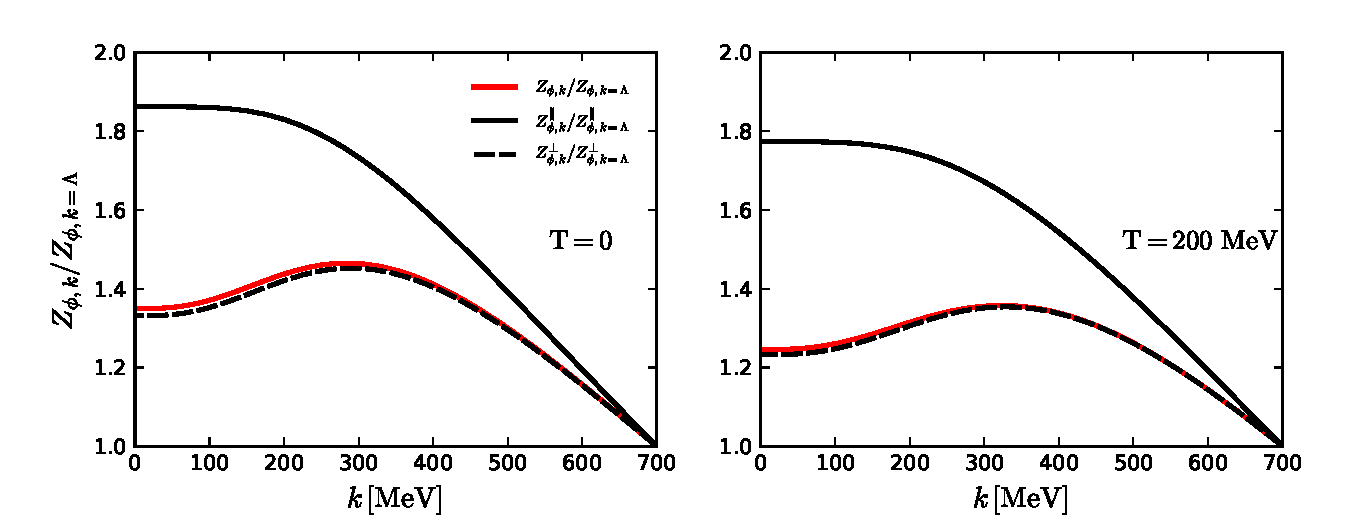
\includegraphics[width=1\textwidth]{zphi}
\caption{Transversal and longitudinal wave function renormalizations for the mesons, $Z_{\phi,k}^{\perp}$, $Z_{\phi,k}^{\parallel}$, as functions of the RG scale $k$ in the vacuum (left panel) and at a finite temperature (right panel), in comparison to the case neglecting the splitting, i.e., $Z_{\phi,k}=Z_{\phi,k}^{\perp}=Z_{\phi,k}^{\parallel}$, as the red line shows. Calculations are performed with the fixed point expansion.}\label{fig:zphi}
\end{figure*}
%%%%%%%%%%%%%%%%%%%%%%%%%%%%%
%

%
%%%%%%%%%%%%%%%%%%%%%%%%%%%%%
\begin{figure*}[t]
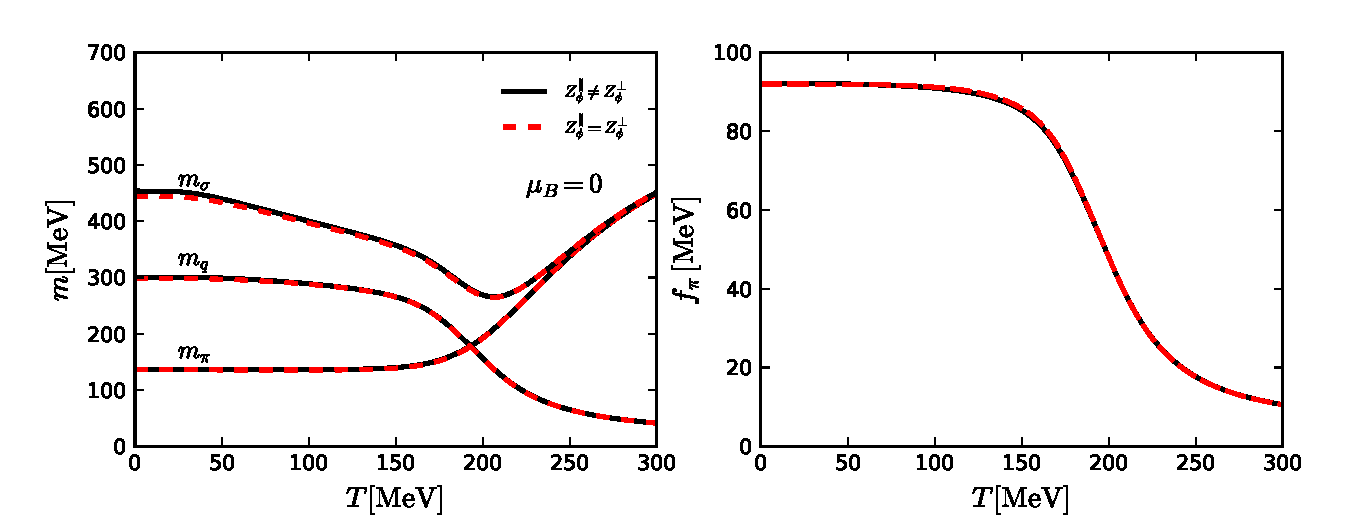
\includegraphics[width=1\textwidth]{mfpi}
\caption{Meson and quark masses (left panel) and $f_\pi$ (right panel) as functions of the temperature at $\mu_B=0$. Calculated results with the splitting of the meson wave function renormalization are compared to those without the splitting, i.e., $Z_{\phi,k}^{\perp}=Z_{\phi,k}^{\parallel}$. Calculations are performed with the fixed point expansion.}\label{fig:mfpi}
\end{figure*}
%%%%%%%%%%%%%%%%%%%%%%%%%%%%%
%

%
%%%%%%%%%%%%%%%%%%%%%%%%%%%%%
\begin{figure}[t]
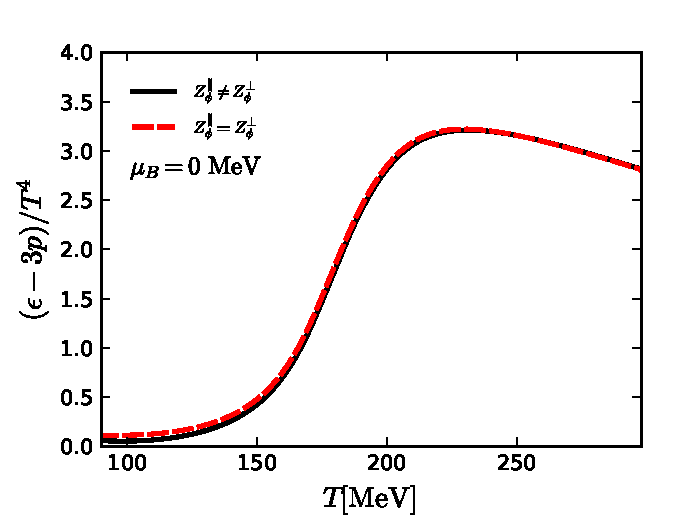
\includegraphics[width=0.5\textwidth]{trace}
\caption{Trace anomaly as a function of the temperature for $\mu_B=0$. Calculated results with and without splitting of the wave function renormalization are presented. Calculations are performed with the fixed point expansion.}\label{fig:trace}
\end{figure}
%%%%%%%%%%%%%%%%%%%%%%%%%%%%%
%

%
%%%%%%%%%%%%%%%%%%%%%%%%%%%%%
\begin{figure*}[t]
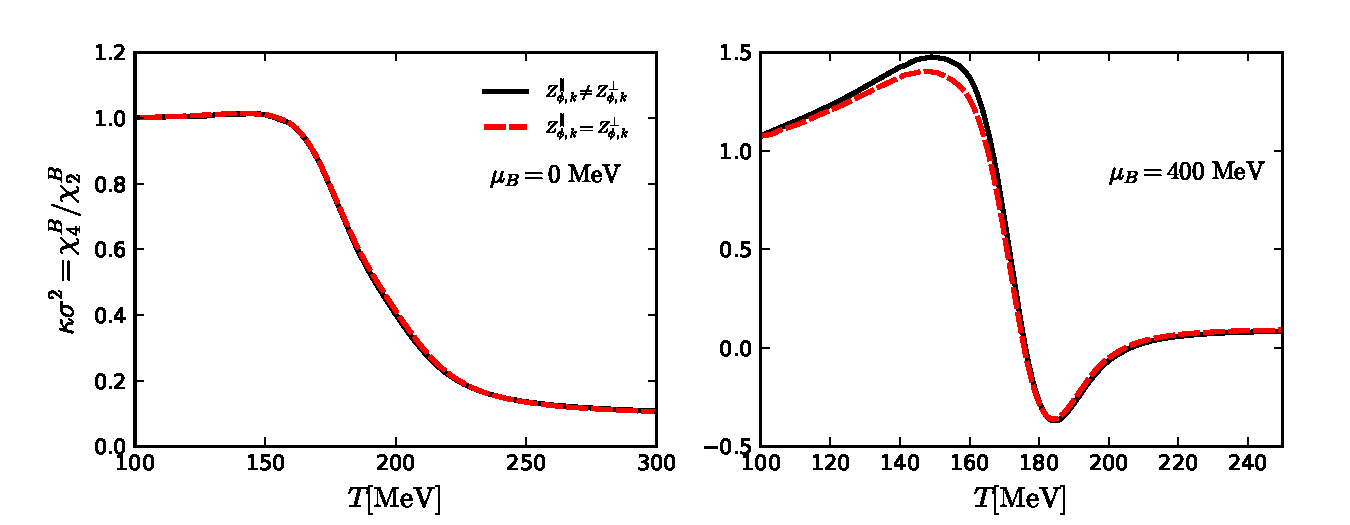
\includegraphics[width=1\textwidth]{kurtosis}
\caption{Kurtosis of the baryon number distribution $\kappa \sigma^2=\chi_4^{B}/\chi_2^{B}$ as a function of the temperature with $\mu_B=0$ (left panel) and $\mu_B=400$ MeV (right panel).  We compare the results obtained from the splitting of the meson wave function renormalization with those assuming $Z_{\phi,k}^{\perp}=Z_{\phi,k}^{\parallel}$. Calculations are performed with the approach of the fixed point expansion.}\label{fig:kurtosis}
\end{figure*}
%%%%%%%%%%%%%%%%%%%%%%%%%%%%%
%

%
%%%%%%%%%%%%%%%%%%%%%%%%%%%%%
\begin{figure*}[t]
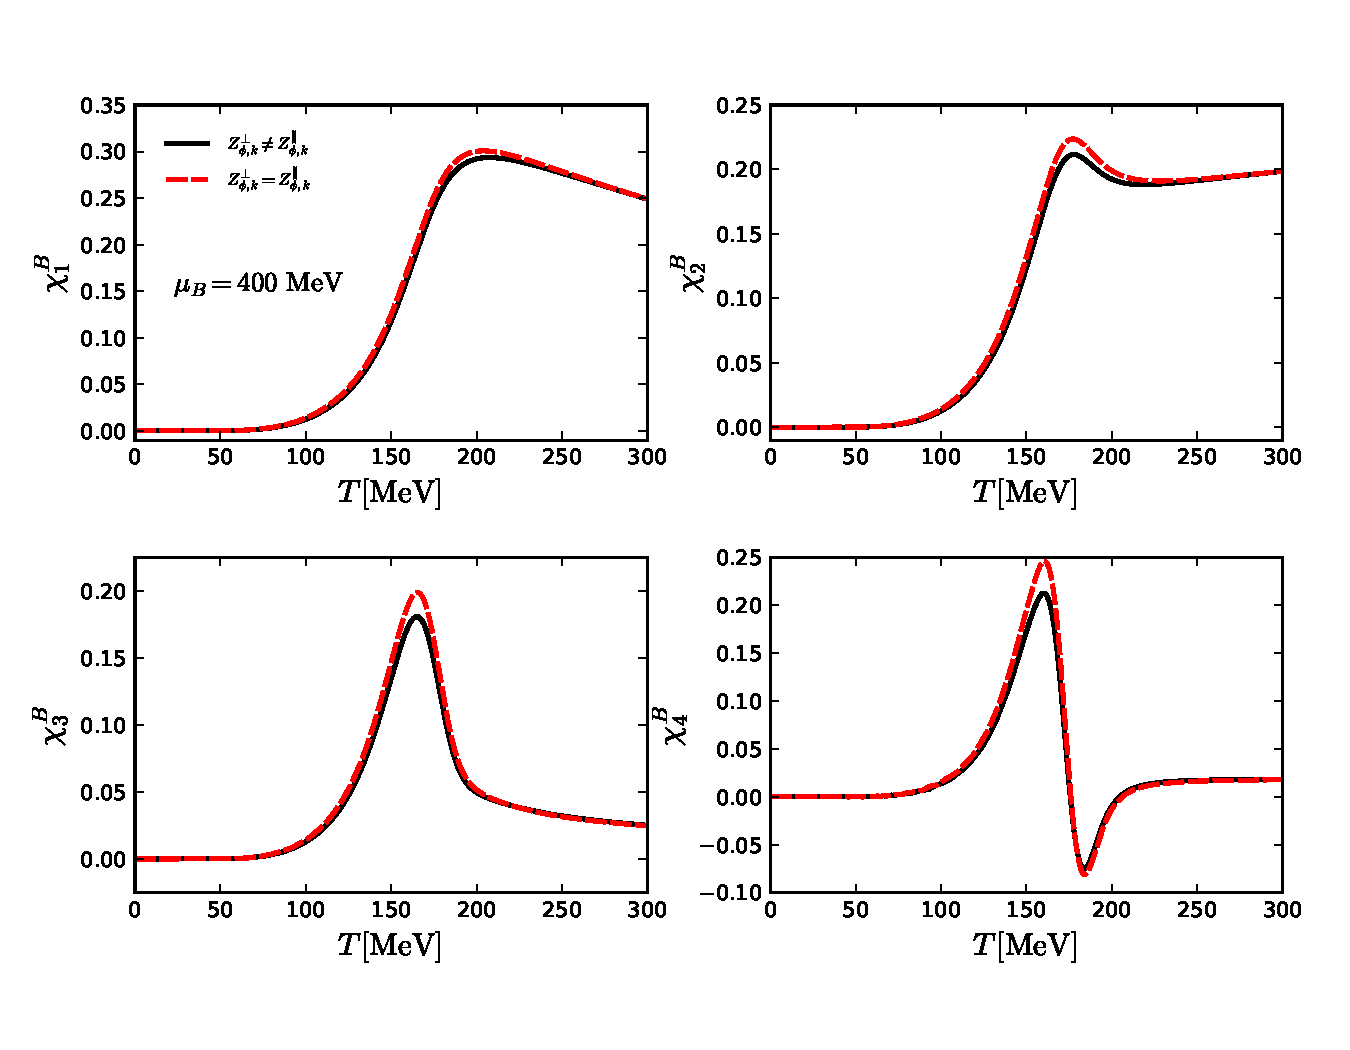
\includegraphics[width=1\textwidth]{chi}
\caption{Fluctuations of the baryon number, $\chi_n^B$'s, up to the fourth order, as functions of the temperature with  $\mu_B=400$ MeV. In the same way, the two cases, $Z_{\phi,k}^{\perp}\ne Z_{\phi,k}^{\parallel}$ and $Z_{\phi,k}^{\perp}=Z_{\phi,k}^{\parallel}$, are compared. Calculations are performed with the approach of the fixed point expansion.}\label{fig:chi}
\end{figure*}
%%%%%%%%%%%%%%%%%%%%%%%%%%%%%
%

We employ the approach of Taylor expansion to solve the flow of the effective potential in \Eq{eq:flowV} numerically. Expanding around the expansion point $\kappa$, one is led to 
\begin{align}\label{}
  V_k(\rho)&=\sum^{N_v}_{n=0}\frac{\lambda_{n,k}}{n!}(\rho-\kappa_k)^n\,,\label{}
\end{align}
where a subscript $k$ is affixed to the expansion point $\kappa$, indicating that the expansion point can be RG scale dependent, and $N_v$ is the highest order which is included in the calculations. The convergency is obtained when the calculated results are almost no longer influenced by the increment of $N_v$, after it is above some value. We adopt two commonly used expansion approaches in the literatures. It is more convenient to work with the renormalized variables, to wit,
\begin{align}
  \bar V_k(\bar \rho)&=\sum^{N_v}_{n=0}\frac{\bar \lambda_{n,k}}{n!}(\bar \rho-\bar \kappa_k)^n\,,\label{eq:barVk}
\end{align}
with $\bar V_k(\bar \rho)=V_k(\rho)$, $\bar \lambda_{n,k}=\lambda_{n,k}/(Z^{\perp}_{\phi,k})^n$, $\bar \rho=Z^{\perp}_{\phi,k} \rho$, and $\bar \kappa_k=Z^{\perp}_{\phi,k}\kappa_k$. Inserting \Eq{eq:barVk} into its flow equation (\ref{eq:flowV}), one is led to
\begin{align}
  &\partial^n_{\bar \rho}\left(\partial_t\big|_{\rho} \bar V_k(\bar \rho)\right)\Big|_{\bar \rho=\bar \kappa_k}\nonumber\\[2ex]
=&(\partial_t -n\eta_{\phi,k}^{\perp})\bar{\lambda}_{n,k}-(\partial_t \bar \kappa_k+\eta_{\phi,k}^{\perp}\bar \kappa_k)\bar \lambda_{n+1,k}\,.\label{eq:drhoV}
\end{align}
Two different expansion approaches are commonly used in the literature: one is the fixed bare expansion point with $\partial_t \kappa_k=0$, i.e., $\kappa_k$ is independent of the scale, which yields 
\begin{align}
  \partial_t \bar \kappa_k+\eta_{\phi,k}^{\perp}\bar \kappa_k&=0\,.\label{eq:dtkappafix}
\end{align}
It follows immediately that the second term on the r.h.s. of \Eq{eq:drhoV} is vanishing for the fixed point expansion. Consequently, $\bar \lambda_{n,k}$'s of different orders are decoupled and there is no feedback from the high order coupling to low order flows. Therefore,  the convergency property is well controlled in the fixed point expansion. For more discussions about the fixed point expansion, see, e.g. \cite{Pawlowski:2014zaa}. Another approach is the running physical expansion, which demands that the expansion point is the solution of equation of motion for every value of $k$, to wit,
\begin{align}
  \frac{\partial}{\partial \bar \rho}\Big(\bar V_k(\bar \rho)-\bar c_k (2\bar \rho)^{\frac{1}{2}}\Big)\bigg|_{\bar \rho=\bar \kappa_k}&=0\,,\label{eq:eosrho}
\end{align}
with $\bar c_k=c/(Z^{\perp}_{\phi,k})^{1/2}$ being the renormalized strength of the explicit chiral symmetry breaking in the effective action \eq{eq:action}. Note that the bare $c$ is scale independent, thus one has $\partial_t \bar c_k=(1/2)\eta_{\phi,k}^{\perp}\bar c_k$. Combining \Eq{eq:drhoV} and \Eq{eq:eosrho}, 
one arrives at the flow of the physical expansion point, which reads
\begin{align}
  \partial_t \bar \kappa_k&=-\frac{\bar c_k^2}{\bar{\lambda}_{1,k}^3+\bar c_k^2\bar{\lambda}_{2,k}}\bigg[\partial_{\bar \rho}\left(\partial_t\big|_{\rho} \bar V_k(\bar \rho)\right)\Big|_{\bar \rho=\bar \kappa_k}\nonumber \\[2ex]
          &+\eta_{\phi,k}^{\perp}\left(\frac{\bar{\lambda}_{1,k}}{2}+\bar\kappa_k\bar{\lambda}_{2,k}\right)\bigg]\,.\label{}
\end{align}
In this work, we will investigate the influence of these two expansion approaches on the fluctuations of the baryon number. 

Furthermore, we also use the Taylor expansion to include the field dependence of the Yukawa coupling, which reads
\begin{align}
  \bar h_k(\bar \rho)&=\sum^{N_h}_{n=0}\frac{\bar h_{n,k}}{n!}(\bar \rho -\bar \kappa_k)^n\,,\label{}
\end{align}
with 
\begin{align}
  \bar h_k(\bar \rho)&=\frac{h_k(\rho)}{Z_{q,k}(Z^{\perp}_{\phi,k})^{1/2}}\,,\quad \text{and}\quad \bar h_{n,k}=\frac{h_{n,k}}{Z_{q,k}(Z^{\perp}_{\phi,k})^{(2n+1)/2}}\,,\label{eq: barhk}
\end{align}
where $N_h$ is the order, up to which the Taylor expansion of $\bar h_k(\bar \rho)$ is done. Inserting \Eq{eq: barhk} into \Eq{eq:dth}, one is led to
\begin{align}
  &\partial^n_{\bar \rho}\left(\partial_t\big|_{\rho} \bar h_k(\bar \rho)\right)\Big|_{\bar \rho=\bar \kappa_k}\nonumber\\[2ex]
=&(\partial_t -n\eta_{\phi,k}^{\perp})\bar h_{n,k}-(\partial_t \bar \kappa_k+\eta_{\phi,k}^{\perp}\bar \kappa_k)\bar h_{n+1,k}\,,\label{}
\end{align}
through which the Yukawa couplings of high orders can be solved.

It is left to specify the parameters in the low energy effective models: the UV cutoff is chosen to be $\Lambda=$ 700 MeV; the effective potential at $k=\Lambda$ is parameterized as follows
\begin{align}
  V_\Lambda(\rho)&=\frac{\lambda_\Lambda}{2}\rho^2+\nu_\Lambda\rho\,,\label{}
\end{align}
with $\lambda_\Lambda=$10 and $\nu_\Lambda=(0.556\,\mathrm{GeV})^2$. Furthermore, the strength of the explicit chiral symmetry breaking in \eq{eq:action} is $c=1.97\times 10^{-3}\,(\mathrm{GeV})^3$, and the Yukawa coupling is $h_\Lambda=7.33$. Employing the fixed point expansion and all the truncations discussed in this work, including the splitting of the meson wave function renormalization and the field dependent Yukawa coupling, etc., we obtain the physical observables in the vacuum, which read $f_\pi=$92 MeV, $m_q=$300 MeV, $m_\pi=$136 MeV, and $m_\sigma=$454 MeV. Note that this is the only set of parameters we use in this work, even they result in some quantitative change of the observables in the vacuum by adopting other truncations discussed in the following. We will not tune these parameters to match the physical observables in the vacuum for different truncations, which would facilitate the comparisons among different truncations.


%%%%%%%%%%%%%%%%%%%%%%%%%%%%%%%%%%%%%%%%%%%%%%%%%%%%%%%%%%%%%
\subsection{Effects of the splitting of the meson wave function renormalization}
\label{sec:splitting}

In this subsection, we investigate the effects of the splitting of meson wave function renormalization on the equation of state (EoS) and the baryon number fluctuations. In order to focus on this research, only the fixed point expansion for the effective potential in \Eq{eq:dtkappafix} is adopted in this subsection.

In \Fig{fig:zphi} we show the running of the transversal and longitudinal wave function renormalizations for the mesons, $Z_{\phi,k}^{\perp}$, $Z_{\phi,k}^{\parallel}$, with the RG scale $k$. The results obtained from the calculation without splitting are also presented for comparison. One can see that the splitting of $Z_{\phi,k}^{\perp}$ and $Z_{\phi,k}^{\parallel}$ takes place even in the vacuum, which is attributed to $3d$ regulators used in this work, as shown in \Eq{eq:Rphi} and \Eq{eq:Rq}, which break the $O(4)$ symmetry. We also find that when the splitting is not taken into account, which is usually adopted in the literature, the difference between $Z_{\phi,k}$ and $Z_{\phi,k}^{\perp}$ is very small. Note that $Z_{\phi,k}$ here is also derived from the spacial component, see \Eq{eq:etaphiperp}. Even though, the small difference between $Z_{\phi,k}$ and $Z_{\phi,k}^{\perp}$ has already indicated that the approximation neglecting the splitting is reasonable. In \Fig{fig:mfpi} we investigate the influence of the splitting of the meson wave function renormalization on the  meson, quark masses and $f_\pi$. One observes that there is almost no difference between the two cases with and without splitting, except for a small effect for the $\sigma$-meson mass in the low temperature regime. In \Fig{fig:trace} we plot the trace anomaly as a function of the temperature with $\mu_B=0$. In the same way, we compare the results with and without splitting of the meson wave function renormalization, and the results show that the effect of the splitting on the trace anomaly is small.

In \Fig{fig:kurtosis} we investigate the influence of the splitting meson wave function on the kurtosis of the baryon number distribution, i.e., $\kappa \sigma^2=\chi_4^{B}/\chi_2^{B}$. One observes that when the baryon chemical potential is vanishing, the two calculations give almost identical results. With the increase of the chemical potential, e.g., $\mu_B=400$ MeV, as shown in the right panel of \Fig{fig:kurtosis}, the splitting meson wave function has begun to play a role, and there is difference between the two calculations, especially in the region near the phase transition. In order to find where the difference comes from. We present the fluctuations of the baryon number of different orders at $\mu_B=400$ MeV in \Fig{fig:chi}. One can see that the fluctuations of the baryon number of all the orders show here, has been suppressed a bit by the splitting of the meson wave function renormalization during the chiral phase transition. But the magnitude of the difference is mild.

In a short summary,  in this section we have investigated the influences of the splitting meson wave function renormalization on the phase transition, QCD thermodynamics and EoS, and the fluctuations of the baryon number. We find that the influences are very small, except that for the baryon number fluctuations at large baryon chemical potential, even there, the difference is just mild. Therefore, we conclude that the splitting of the meson wave function renormalization can be safely neglected in the studies of equilibrium thermodynamical bulk properties within the low energy effective model. However, we should remind that the situation may be different when the nonequilibrium properties, 




 



































%%%%%%%%%%%%%%%%%%%%%%%%%%%%%%%%%%%%
\acknowledgments
Thanks


%%%%%%%%%%%%%%%%%%%%%%%%%%%%%%%%%%%%%%%%%%%%%%%%%%%%%%%%%%%%%
%%%%%%%%%%%%%%%%%%%%%%%%%%%%%%%%%%%%%%%%%%%%%%%%%%%%%%%%%%%%%

\appendix

\section{Anomalous dimensions and Yukawa coupling}
\label{app:anom}

Inserting the effective action in \Eq{eq:action} and its the flow equation in \Eq{eq:WetterichEqPQM} into \Eq{eq:etaphiperp}, and employing the $3d$- regulators in \Eq{eq:Rphi} and \Eq{eq:Rq}, one obtains the transversal anomalous dimension for the meson, as follows
\begin{align}
  \eta_{\phi,k}^{\perp}&=\frac{1}{6\pi^2}\Bigg\{\frac{4}{k^2 z_\phi^4} \bar{\kappa}_k(\bar{V}''_k(\bar{\kappa}_k))^2\mathcal{BB}_{(2,2)}(\bar{m}^{2}_{\pi,k},\bar{m}^{2}_{\sigma,k};T)\nonumber\\[2ex]
&+N_c\bar{h}^{2}_{k}\bigg[\mathcal{F}_{(2)}(\bar{m}^{2}_{q,k};T,\mu)(2\eta_{q,k}-3)\nonumber\\[2ex]
&-4(\eta_{q,k}-2)\mathcal{F}_{(3)}(\bar{m}^2_{q,k};T,\mu)\bigg]\Bigg\}\,, \label{eq:etaphiperp2}  
\end{align} 
and relevant threshold functions are given in \app{app:thresholdfun}. In the same way, the longitudinal anomalous dimension for the meson in \Eq{eq:etaphipara} reads
\begin{align}
  \eta_{\phi,k}^{\parallel}&=\frac{1}{6\pi^2}\Bigg\{\frac{4}{k^2 z_\phi^4}\bar{\kappa}_k(\bar{V}''_k(\bar{\kappa}_k))^2\bigg[-6\mathcal{BB}_{(2,2)}(\bar{m}^{2}_{\pi,k},\bar{m}^{2}_{\sigma,k};T)\nonumber\\[2ex]
&+\frac{4}{z_\phi}(1+\bar{m}^{2}_{\sigma}){\mathcal{BB}}_{(2,3)}(\bar{m}^{2}_{\pi,k},\bar{m}^{2}_{\sigma,k};T)\nonumber\\[2ex]
&+\frac{4}{z_\phi}(1+\bar{m}^{2}_{\pi}){\mathcal{BB}}_{(3,2)}(\bar{m}^{2}_{\pi,k},\bar{m}^{2}_{\sigma,k};T)\bigg]\nonumber\\[2ex]
&\times(1-\frac{1}{5}\eta^{\bot}_{\phi,k})+\frac{N_c\bar{h}^{2}_{k}}{z_\phi}\mathcal{F}_{(3)}(\bar{m}^{2}_{q,k};T,\mu)(4-\eta_{q,k})\bigg\}\,, \label{eq:etaphipara2}  
\end{align} 

The anomalous dimension for the quark in \Eq{eq:etapsi} is given by
\begin{align}
\eta_{q,k}=&\frac{1}{24\pi^2N_f}(4-\eta_{\phi,k}^{\perp})\bar{h}^{2}_{k}\nonumber\\[2ex]
&\times\bigg\{ (N^{2}_{f}-1)\mathcal{FB}_{(1,2)}(\bar{m}^{2}_{q,k},\bar{m}^{2}_{\pi,k};T,\mu,p_{0,ex})\nonumber\\[2ex]
&+\mathcal{FB}_{(1,2)}(\bar{m}^{2}_{q,k},\bar{m}^{2}_{\sigma,k};T,\mu,p_{0,ex})\bigg\}\,, \label{eq:etapsi2}
\end{align} 
where $p_{0,ex}=\pi T$ for the finite temperature part and $\big[k^2+(\pi T)^2\exp\{-2k/(5 T)\}\big]^{1/2}$ for the vacuum part in the threshold function $\mathcal{FB}$'s in \Eq{eq:FB}. Note that the modification of the lowest-order Matsubara frequency in the vacuum part is employed to suppress the artificial temperature dependence of thermodynamics in the low temperature regime, see e.g. \cite{Fu:2015naa,Fu:2016tey} for more discussions. The flow of the field-dependent Yukawa coupling in \Eq{eq:dth} is firstly derived in \cite{Pawlowski:2014zaa} and is also presented here for convenience, which reads
\begin{align}
  \partial_t&\big|_{\rho}\bar{h}_k(\bar{\rho})=\left(\frac{1}{2}\eta_{\phi,k}+\eta_{q,k}\right)\bar{h}_k(\bar{\rho})\nonumber\\[2ex]
&+\frac{\bar{h}^3_k(\bar{\rho})}{4\pi^2N_f}\bigg[L^{(4)}_{(1,1)}(\bar{m}^{2}_{q,k},\bar{m}^{2}_{\sigma,k},\eta_{q,k},\eta_{\phi,k}^{\perp};T,\mu,p_{0,ex})\nonumber\\[2ex]
&-(N^{2}_{f}-1)L^{(4)}_{(1,1)}(\bar{m}^{2}_{q,k},\bar{m}^{2}_{\pi,k},\eta_{q,k},\eta_{\phi,k}^{\perp};T,\mu,p_{0,ex})\bigg]\nonumber\\[2ex]
&+\frac{1}{2\pi^2}\bar{h}_k(\bar{\rho})\bar{h}'_k(\bar{\rho})\bar{\rho}\bigg[\bar{h}_k(\bar{\rho})+\bar{\rho}\bar{h}'_k(\bar{\rho})\bigg]\nonumber\\[2ex]
&\times L^{(4)}_{(1,1)}(\bar{m}^{2}_{q,k},\bar{m}^{2}_{\sigma,k},\eta_{q,k},\eta_{\phi,k}^{\perp};T,\mu,p_{0,ex})\nonumber\\[2ex]
&-\frac{k^2}{4\pi^2}\bigg[\left(3\bar{h}'_k(\bar{\rho})+2\bar{\rho}\bar{h}''_k(\bar{\rho})\right)l^{(B,4)}_{1}(\bar{m}^{2}_{\sigma,k},\eta_{\phi,k}^{\perp};T)\nonumber\\[2ex]
&+3\bar{h}'_k(\bar{\rho})l^{(B,4)}_{1}(\bar{m}^{2}_{\pi,k},\eta_{\phi,k}^{\perp};T)\bigg]\,.\label{eq:dth2}  
\end{align} 



%%%%%%%%%%%%%%%%%%%%%%%%%%%%%%%%%%%%
\section{Threshold functions}
\label{app:thresholdfun}


In this work we use the $3d$- flat or Litim regulators \cite{Litim:2000ci,Litim:2001up}, which are very suited for the computations at finite temperature and densities, since the summation for the Matsubara frequencies is not affected by the $3d$ regulators, and can be performed analytically. The regulators in \Eq{eq:WetterichEqPQM} read
\begin{align}
  R^{\phi}_{k}(q_0,\bm{q})&=Z^{\perp}_{\phi,k}\bm{q}^2 r_B(\bm{q}^2/k^2)\,, \label{eq:Rphi}\\[2ex] 
  R^{q}_{k}(q_0,\bm{q})&=Z_{q,k}i\bm{\gamma} \cdot \bm{q} r_F(\bm{q}^2/k^2)\,, \label{eq:Rq}
\end{align} 
with 
\begin{align}
  r_B(x)&=\left( \frac{1}{x}-1 \right)\Theta(1-x)\,,\\[2ex] 
  r_F(x)&=\left( \frac{1}{\sqrt{x}}-1 \right)\Theta(1-x)\,,  \label{}
\end{align} 
where $\Theta(x)$ is the Heaviside step function. Note that since $Z^{\perp}_{\phi,k}\neq Z^{\parallel}_{\phi,k}$, it is  the transversal wave function renormalization for the meson appearing in \Eq{eq:Rphi}.

In the threshold functions we usually need the dimensionless meson and quark propagators as follows
\begin{align}
  G_\phi(q,\bar{m}^{2}_{\phi,k})&=\frac{1}{z_\phi\tilde{q}^{2}_{0}+1+\bar{m}^{2}_{\phi,k}}\,, \label{eq:Gphi}\\[2ex] 
  G_q(q,\bar{m}^{2}_{q,k})&=\frac{1}{(\tilde{q}_0+i\tilde{\mu})^2+1+\bar{m}^{2}_{q,k}}\,, \label{eq:Gq}
\end{align} 
with $\tilde{\mu}=\mu/k$ and $\tilde{q}_0=q_0/k$, where the Matsubara frequency is  $q_0=2n_q\pi  T$ for bosons and $(2n_q+1)\pi T $ for fermions with $n_q\in \mathbb{Z}$.

The definition of the threshold functions $\mathcal{B}_{(n)}$ and $\mathcal{F}_{(n)}$ is given by
\begin{align}
  \mathcal{B}_{(n)}(\bar{m}^{2}_{\phi,k};T)&=\frac{T}{k}\sum_{n_q}\Big(G_{\phi}(q,\bar{m}^{2}_{\phi,k})\Big)^n\,,\label{eq:Bn} \\[2ex]
  \mathcal{F}_{(n)}(\bar{m}^{2}_{q,k};T,\mu)&=\frac{T}{k}\sum_{n_q}\Big(G_q(q,\bar{m}^{2}_{q,k})\Big)^n\,.\label{eq:Fn}
\end{align}
After performing the Matsubara sum, one arrives at
\begin{align}
    \mathcal{B}_{(1)}(\bar{m}^{2}_{\phi,k};T)=&\frac{1}{\sqrt{z_\phi(1+\bar{m}^{2}_{\phi,k})}}\bigg(\frac{1}{2}+n_{B}(\bar{m}^{2}_{\phi,k},z_\phi;T)\bigg)\,,\label{eq:B1}
\end{align}
and
\begin{align}
    &\mathcal{F}_{(1)}(\bar{m}^{2}_{q,k};T,\mu)=\frac{1}{2\sqrt{1+\bar{m}^{2}_{q,k}}}\nonumber\\[2ex]
    &\hspace{.3cm}\times\Big(1-n_{F}(\bar{m}^{2}_{q,k};T,\mu)-n_{F}(\bar{m}^{2}_{q,k};T,-\mu)\Big)\,,\label{eq:F1}
\end{align}
with the bosonic and fermionic distribution functions being
\begin{align}
  n_B(\bar{m}^{2}_{\phi,k},z_\phi;T)&=\frac{1}{\exp\bigg\{\frac{1}{T}\frac{k}{z_\phi^{1/2}}\sqrt{1+\bar{m}^{2}_{\phi,k}}\bigg\}-1}\,,
\end{align} 
and
\begin{align}
  n_F(\bar{m}^{2}_{q,k};T,\mu)&=\frac{1}{\exp\bigg\{\frac{1}{T}\Big[k\sqrt{1+\bar{m}^{2}_{q,k}}-\mu\Big]\bigg\}+1}\,.
\end{align} 
Note that when the Polaykov loop is taken into account, the fermionic distribution function is modified as follows
\begin{align}
n_F(\bar{m}^{2}_{q,k};T,\mu,L,\bar{L})&=\frac{1+2\bar{L}e^{x/T}+Le^{2x/T}}{1+3\bar{L}e^{x/T}+3Le^{2x/T}+e^{3x/T}}\,,
\end{align} 
with $x=k\sqrt{1+\bar{m}^{2}_{q,k}}-\mu$, and $n_{F}(\bar{m}^{2}_{q,k};T,-\mu)$ in \Eq{eq:F1} is replaced with $n_F(\bar{m}^{2}_{q,k};T,-\mu,\bar L, L)$ accordingly. With \Eq{eq:B1} and \Eq{eq:F1}, high-order threshold functions in Eqs. (\ref{eq:Bn}) and (\ref{eq:Fn}) are readily obtained as
\begin{align}
  \mathcal{B}_{(n+1)}(\bar{m}^{2}_{\phi,k};T)&=-\frac{1}{n}\frac{\partial}{\partial \bar{m}^{2}_{\phi,k}}\mathcal{B}_{(n)}(\bar{m}^{2}_{\phi,k};T)\,,\\[2ex]
  \mathcal{F}_{(n+1)}(\bar{m}^{2}_{q,k};T,\mu)&=-\frac{1}{n}\frac{\partial}{\partial \bar{m}^{2}_{q,k}}
                                    \mathcal{F}_{(n)}(\bar{m}^{2}_{q,k};T,\mu)\,. 
\end{align}

The threshold functions in the flow of effective potential in \Eq{eq:flowV} are given by
\begin{align}
  &l_0^{(B,d)}(\bar{m}^{2}_{\phi,k},\eta^\perp_{\phi,k},z_\phi;T)\nonumber\\[2ex]
  =&\frac{2}{d-1}\left( 1- \frac{\eta^{\bot}_{\phi,k}}{d+1}\right)\mathcal{B}_{(1)}(\bar{m}^{2}_{\phi,k},z_\phi;T)\,,\label{eq:l0B}
\end{align} 
and
\begin{align}
  &l_0^{(F,d)}(\bar{m}^{2}_{q,k},\eta_{q,k};T,\mu)\nonumber\\[2ex]
  =&\frac{2}{d-1}\left( 1-\frac{\eta_{q,k}}{d} \right)\mathcal{F}_{(1)}(\bar{m}^{2}_{q,k};T,\mu)\,.\label{eq:l0F}
\end{align} 
In \Eq{eq:dth2}, one also needs $l^{(B,4)}_{1}$, which is obtained from 
\begin{align}
  l_1^{(B/F,d)}(m^{2})=&-\frac{\partial}{\partial m^{2}}l_0^{(B/F,d)}(m^{2})\,.\label{}
\end{align} 

Furthermore, we also need other threshold functions, such as
\begin{align}
  &\mathcal{BB}_{(n_1,n_2)}(m_1^2,m_2^2;T)\nonumber\\[2ex]
=&\frac{T}{k}\sum_{n_q}\Big(G_\phi(q,\bar{m}^{2}_{\phi_a,k})\Big)^{n_1} \Big(G_\phi(q,\bar{m}^{2}_{\phi_b,k})\Big)^{n_2}\,.\label{eq:BBn1n2}
\end{align}
in the expressions of the mesonic anomalous dimension in Eqs. (\ref{eq:etaphiperp}) and (\ref{eq:etaphipara}). Inserting \Eq{eq:Gphi} into \Eq{eq:BBn1n2}, one is led to
\begin{align}
  &\mathcal{BB}_{(1,1)}(\bar{m}^{2}_{\phi_a,k},\bar{m}^{2}_{\phi_b,k};T)\nonumber\\[2ex]
  =&-\frac{1}{z^{1/2}_{\phi}}\Bigg\{\left(\frac{1}{2}+n_B(\bar{m}^{2}_{\phi_a,k},z_\phi;T) \right)\frac{1}{(1+\bar{m}^{2}_{\phi_a,k})^{1/2}} \nonumber\\[2ex]
&\times \frac{1}{\bar{m}^{2}_{\phi_a,k}-\bar{m}^{2}_{\phi_b,k}}+\left( \frac{1}{2}+n_B(\bar{m}^{2}_{\phi_b,k},z_\phi;T) 
\right)\nonumber\\[2ex]
&\times \frac{1}{(1+\bar{m}^{2}_{\phi_b,k})^{1/2}}\frac{1}{\bar{m}^{2}_{\phi_b,k}-\bar{m}^{2}_{\phi_a,k}}\Bigg\}\,.\label{eq:BB11}
\end{align} 
In the same way, one could obtain higher-order ones by employing, e.g.,
\begin{align}
  &\mathcal{BB}_{(n_1+1,n_2)}(\bar{m}^{2}_{\phi_a,k},\bar{m}^{2}_{\phi_b,k};T)\nonumber\\[2ex]
  =&-\frac{1}{n_1}\frac{\partial}{\partial \bar{m}^{2}_{\phi_a,k}}\mathcal{BB}_{(n_1,n_2)}(\bar{m}^{2}_{\phi_a,k},\bar{m}^{2}_{\phi_b,k};T)\,.
\end{align}

In the flow of the Yukawa coupling in (\ref{eq:dth}), the threshold function $L$ is introduced, which reads
\begin{align}
  &L^{(4)}_{(1,1)}(\bar{m}^{2}_{q,k},\bar{m}^{2}_{\phi,k},\eta_{q,k},\eta_{\phi,k};T,\mu,p_0)\nonumber\\[2ex]
  =&\frac{2}{3}\bigg[\left(1-\frac{\eta_{\phi,k}^{\perp}}{5}\right)\mathcal{FB}_{(1,2)}(\bar{m}^{2}_{q,k},\bar{m}^{2}_{\phi,k};T,\mu,p_0)\nonumber\\[2ex]
&+\left(1-\frac{\eta_{q,k}}{4}\right)\mathcal{FB}_{(2,1)}(\bar{m}^{2}_{q,k},\bar{m}^{2}_{\phi,k};T,\mu,p_0)\bigg]\,,
\end{align} 
where the fermionic and bosonic mixing threshold functions $\mathcal{FB}$'s are given by
\begin{align}
 &\mathcal{FB}_{(n_f,n_b)}(\bar{m}^{2}_{q,k},\bar{m}^{2}_{\phi,k};T,\mu,p_0)\nonumber \\[2ex] 
  =&\frac{T}{k}\sum_{n_q}\Big(G_{q}(q,\bar{m}^{2}_{q,k})\Big)^{n_f}\Big(G_{\phi}(q-p,\bar{m}^{2}_{\phi,k})\Big)^{n_b}\,.\label{eq:FB}
\end{align}
The explicit expression for $\mathcal{FB}_{(1,1)}$ is readily obtained after summing the Matsubara frequency, which can be found in, e.g. \cite{Fu:2015naa}. Higher-order $\mathcal{FB}$'s are obtained from $\mathcal{FB}_{(1,1)}$ by performing derivatives w.r.t. relevant masses as same as other threshold functions mentioned above.

%%%%%%%%%%%%%%%%%%%%%%%%%%%%%%%%%%%%%%%%%%%%




%%%%%%%%%%%%%%%%%%%%%%%%%%%%%%%%%%%%%%%%%%%%

% The \nocite command causes all entries in a bibliography to be
% printed out whether or not they are actually referenced in the
% text. This is appropriate for the sample file to show the different
% styles of references, but authors most likely will not want to use
% it.  \nocite{*}

%\bibliography{refspec}% Produces the bibliography via BibTeX.
\bibliography{ref-lib}% Produces the bibliography via BibTeX.


\end{document}